\documentclass[a4paper, 11pt]{article}
\usepackage[UTF8, scheme = plain]{ctex}
\usepackage{amsmath}
\usepackage{graphicx}
\usepackage{geometry}
\usepackage{listings}
\geometry{scale=0.8}
\linespread{1.5}
\usepackage{hyperref}


\title{	
\normalfont \normalsize
\textsc{School of Data and Computer Science, Sun Yat-sen University} \\ [25pt] %textsc small capital letters
\rule{\textwidth}{0.5pt} \\[0.4cm] % Thin top horizontal rule
\huge  E06 FF Planner \\ % The assignment title
\rule{\textwidth}{2pt} \\[0.5cm] % Thick bottom horizontal rule
\author{Suixin Ou \and Yangkai Lin}
\date{\normalsize October 12, 2020}
}

\begin{document}
\maketitle
\tableofcontents
\newpage

\section{Examples}

\subsection{Spare Tire}
\label{sec:spare-tire}

\begin{lstlisting}[title=domain\_spare\_tire.pddl,frame=single,language=lisp,numbers=left]
(define (domain spare_tire)
  (:requirements :strips :equality:typing)
  (:types physob location) 
  (:predicates  (Tire ?x - physob)
		(at ?x - physob ?y - location))

(:action Remove
             :parameters (?x - physob ?y - location)
             :precondition (At ?x ?y)
             :effect (and (not (At ?x ?y)) (At ?x Ground)))

  (:action PutOn
             :parameters (?x - physob)
             :precondition (and (Tire ?x) (At ?x Ground) 
                                (not (At Flat Axle)))
             :effect (and (not (At ?x Ground)) (At ?x Axle)))
  (:action LeaveOvernight
             :effect (and (not (At Spare Ground)) (not (At Spare Axle)) 
                          (not (At Spare Trunk)) (not (At Flat Ground)) 
                          (not (At Flat Axle)) (not (At Flat Trunk)) ))
 )

\end{lstlisting}
\begin{lstlisting}[title=spare\_tire.pddl,frame=single,language=lisp,numbers=left]
(define (problem prob)
 (:domain spare_tire)
 (:objects Flat Spare -physob Axle Trunk Ground - location)
 (:init (Tire Flat)(Tire Spare)(At Flat Axle)(At Spare Trunk))
 (:goal (At Spare Axle))
)


\end{lstlisting}
\begin{figure}[h]
  \centering
  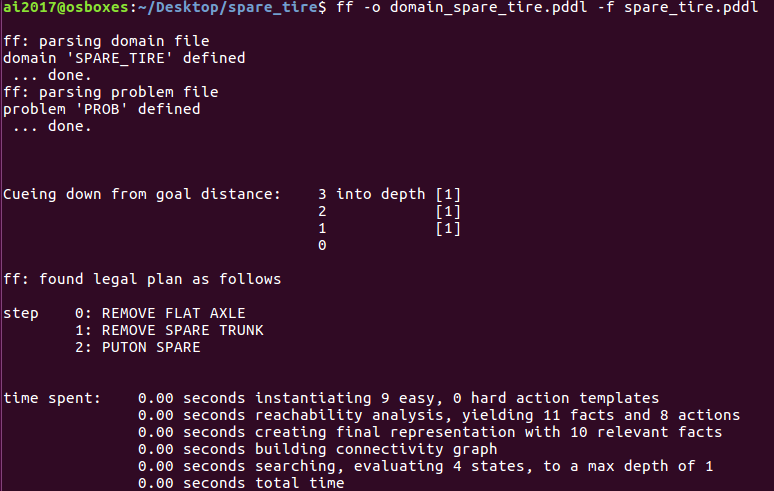
\includegraphics[width=16cm]{Pic/spare_tire}
\end{figure}

\subsection{Briefcase World}
\label{sec:briefcase-world}

Please refer to \texttt{pddl.pdf} at page 2. Please pay More attention to the usages of \texttt{forall} and \texttt{when}.  

For more examples, please refer to \texttt{ff-domains.tgz} and \texttt{benchmarksV1.1.zip}. For more usages of FF planner, please refer to the documentation \texttt{pddl.pdf}.
\section{Tasks}

\subsection{8-puzzle}
\begin{figure}[ht]
  \centering
  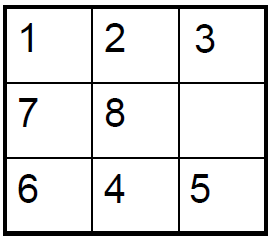
\includegraphics[width=0.4\textwidth]{Pic/puzzle}
  \qquad
  \parbox[b]{0.4\textwidth}{Please complete  \texttt{domain\_puzzle.pddl} and \texttt{puzzle.pddl} to solve the 8-puzzle problem.\\}
\end{figure}
\label{sec:8-puzzle}
\begin{lstlisting}[title=domain\_puzzle.pddl,frame=single,language=lisp,numbers=left]
(define (domain puzzle)
  (:requirements :strips :equality:typing)
  (:types num loc) 
  (:predicates  ())

(:action slide
             :parameters ()
             :precondition ()
             :effect () 
 )
)
\end{lstlisting}
\begin{lstlisting}[title=domain\_puzzle.pddl,frame=single,language=lisp,numbers=left]
(define (problem prob)
 (:domain puzzle)
 (:objects )
 (:init )
 (:goal ())
)

\end{lstlisting}
\subsection{Blocks World}
Planning in the blocks world is a traditional planning exercise, and you can recall what we have introduced in the theory course.
\\ There are a collection of blocks: a block can be on the table, or on the top of another block. 
\\ There are three predicates:  
\begin{itemize}

\item\textit{clear(x)}: there is no block on top of block x;

\item \textit {on(x,y)}: block x is on the top of block y;

\item   \textit {onTable(x)}: block x is on the table

\end{itemize}There are two actions in this task:
\begin{itemize}

\item\textit{move(x,y)}: move block x onto block y, provided that both x and y are clear;

\item \textit {moveToTable(x)}: move block x on to the table, provided that x is clear and x is not on the table;

\end{itemize}Give initial state and goal state, find the actions change the initial state to the goal state.
\\
\\
In this task, please complete the file \texttt{domain\_blocks.pddl} to solve the blocks world problem. You should know the usages of \texttt{forall} and \texttt{when}.

\begin{lstlisting}[title=domain\_blocks.pddl,frame=single,language=lisp,numbers=left]
(define (domain blocks)
  (:requirements :strips :typing:equality
                 :universal-preconditions
                 :conditional-effects)
  (:types physob)
  (:predicates   
  	    (ontable ?x - physob)
            (clear ?x - physob)	
	    (on ?x ?y - physob))
		
  (:action move
             :parameters (?x ?y - physob)
             :precondition ()
             :effect ()
             )

  (:action moveToTable
             :parameters (?x - physob)
             :precondition ()
             :effect ( )
 )



\end{lstlisting}

\label{sec:problem-description}

\begin{lstlisting}[title=blocks.pddl,frame=single,language=lisp,numbers=left]
(define (problem prob)
 (:domain blocks)
 (:objects A B C D E F - physob)
 (:init (clear A)(on A B)(on B C)(ontable C) (ontable D)
  (ontable F)(on E D)(clear E)(clear F)
)
 (:goal  (and (clear F) (on F A) (on A C) (ontable C)(clear E) (on E B) 
         (on B D) (ontable D)) )
 )




\end{lstlisting}
Please submit a file named \textsf{E06\_YourNumber.pdf}, and send it to \textsf{ai\_2020@foxmail.com}


\section{Codes and Results}
\subsection{8-puzzle}
\subsubsection{Codes}
\begin{lstlisting}[title=domain-puzzle.pddl,frame=single,language=lisp,numbers=left]
(define (domain puzzle)
    (:requirements :strips :equality:typing)
    (:types num loc)
    (:predicates
        (at ?x - num ?y - loc)
        (adjacent ?x ?y - loc)
    )
    (:action slide
        :parameters (?x - num ?from ?to - loc)
        :precondition (and (at ?x ?from)
                            (at n0 ?to)
                            (adjacent ?from ?to))
        :effect (and (not (at ?x ?from))
                        (not (at n0 ?to))
                        (at n0 ?from)
                        (at ?x ?to))
    )
)
\end{lstlisting}
\begin{lstlisting}[title=puzzle.pddl,frame=single,language=lisp,numbers=left]
(define (problem prob)
    (:domain puzzle)
    (:objects n1 n2 n3 n4 n5 n6 n7 n8 n0 - num
                l11 l12 l13 l21 l22 l23 l31 l32 l33 - loc)
    (:init
        (at n1 l11)
        (at n2 l12)
        (at n3 l13)
        (at n7 l21)
        (at n8 l22)
        (at n0 l23)
        (at n6 l31)
        (at n4 l32)
        (at n5 l33)
        (adjacent l11 l12)
        (adjacent l11 l21)
        (adjacent l12 l11)
        (adjacent l12 l13)
        (adjacent l12 l22)
        (adjacent l13 l12)
        (adjacent l13 l23)
        (adjacent l21 l11)
        (adjacent l21 l22)
        (adjacent l21 l31)
        (adjacent l22 l12)
        (adjacent l22 l21)
        (adjacent l22 l23)
        (adjacent l22 l32)
        (adjacent l23 l13)
        (adjacent l23 l22)
        (adjacent l23 l33)
        (adjacent l31 l21)
        (adjacent l31 l32)
        (adjacent l32 l22)
        (adjacent l32 l31)
        (adjacent l32 l33)
        (adjacent l33 l23)
        (adjacent l33 l32)
    )
    (:goal (and (at n1 l11)
                (at n2 l12)
                (at n3 l13)
                (at n4 l21)
                (at n5 l22)
                (at n6 l23)
                (at n7 l31)
                (at n8 l32)
                (at n0 l33))
    )
)
\end{lstlisting}
\subsubsection{Brief results}
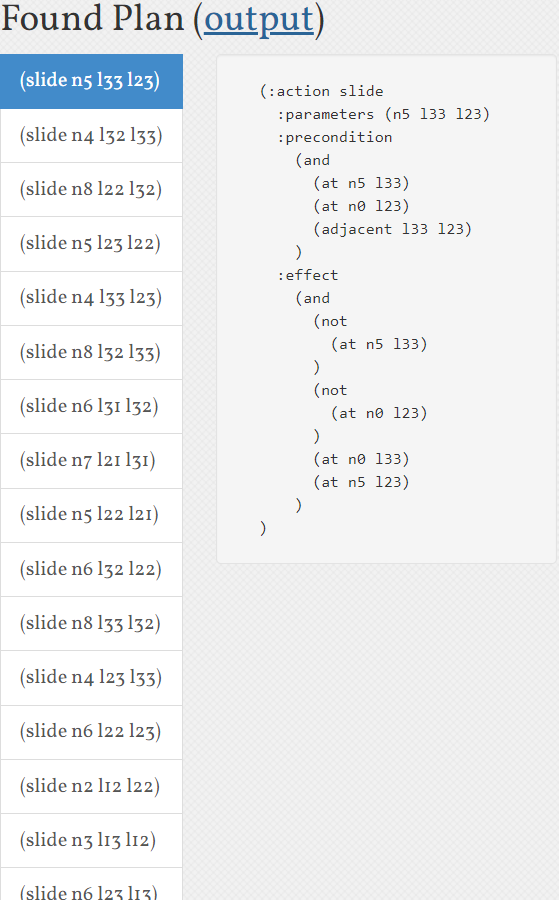
\includegraphics[width=14cm]{result1.png}
\subsubsection{Detailed results}
\begin{lstlisting}[title=result1.txt,frame=single,language=lisp,basicstyle=\tiny]
Executing tests from 1/domain-puzzle.ptest.json.
Planning service: http://solver.planning.domains/solve
Domain: puzzle, Problem: prob
 --- OK.
 Match tree built with 192 nodes.

PDDL problem description loaded: 
	Domain: PUZZLE
	Problem: PROB
	#Actions: 192
	#Fluents: 81
Landmarks found: 9
Starting search with IW (time budget is 60 secs)...
rel_plan size: 11
#RP_fluents 17
Caption
{#goals, #UNnachieved,  #Achieved} -> IW(max_w)

{9/9/0}:IW(1) -> rel_plan size: 11
#RP_fluents 17
{9/6/3}:IW(1) -> [2][3][4]rel_plan size: 9
#RP_fluents 14
{9/5/4}:IW(1) -> [2][3][4][5][6][7][8][9][10][11][12][13][14][15][16][17][18];; NOT I-REACHABLE ;;
Total time: 4.47035e-10
Nodes generated during search: 272
Nodes expanded during search: 263
IW search completed
Starting search with BFS(novel,land,h_add)...
--[4294967295 / 22]--
--[5 / 22]--
--[5 / 20]--
--[5 / 19]--
--[5 / 18]--
--[5 / 16]--
--[5 / 15]--
--[5 / 14]--
--[5 / 11]--
--[5 / 10]--
--[5 / 8]--
--[4 / 8]--
--[3 / 8]--
--[3 / 5]--
--[3 / 2]--
--[2 / 2]--
--[2 / 0]--
--[0 / 0]--
Total time: 0.056
Nodes generated during search: 1484
Nodes expanded during search: 525
Plan found with cost: 61
BFS search completed
0.00100: (slide n5 l33 l23)
0.00200: (slide n4 l32 l33)
0.00300: (slide n8 l22 l32)
0.00400: (slide n5 l23 l22)
0.00500: (slide n4 l33 l23)
0.00600: (slide n8 l32 l33)
0.00700: (slide n6 l31 l32)
0.00800: (slide n7 l21 l31)
0.00900: (slide n5 l22 l21)
0.01000: (slide n6 l32 l22)
0.01100: (slide n8 l33 l32)
0.01200: (slide n4 l23 l33)
0.01300: (slide n6 l22 l23)
0.01400: (slide n2 l12 l22)
0.01500: (slide n3 l13 l12)
0.01600: (slide n6 l23 l13)
0.01700: (slide n4 l33 l23)
0.01800: (slide n8 l32 l33)
0.01900: (slide n2 l22 l32)
0.02000: (slide n4 l23 l22)
0.02100: (slide n6 l13 l23)
0.02200: (slide n3 l12 l13)
0.02300: (slide n4 l22 l12)
0.02400: (slide n5 l21 l22)
0.02500: (slide n1 l11 l21)
0.02600: (slide n4 l12 l11)
0.02700: (slide n5 l22 l12)
0.02800: (slide n2 l32 l22)
0.02900: (slide n7 l31 l32)
0.03000: (slide n1 l21 l31)
0.03100: (slide n4 l11 l21)
0.03200: (slide n5 l12 l11)
0.03300: (slide n2 l22 l12)
0.03400: (slide n4 l21 l22)
0.03500: (slide n1 l31 l21)
0.03600: (slide n7 l32 l31)
0.03700: (slide n4 l22 l32)
0.03800: (slide n1 l21 l22)
0.03900: (slide n5 l11 l21)
0.04000: (slide n2 l12 l11)
0.04100: (slide n1 l22 l12)
0.04200: (slide n5 l21 l22)
0.04300: (slide n2 l11 l21)
0.04400: (slide n1 l12 l11)
0.04500: (slide n5 l22 l12)
0.04600: (slide n4 l32 l22)
0.04700: (slide n7 l31 l32)
0.04800: (slide n2 l21 l31)
0.04900: (slide n4 l22 l21)
0.05000: (slide n5 l12 l22)
0.05100: (slide n1 l11 l12)
0.05200: (slide n4 l21 l11)
0.05300: (slide n2 l31 l21)
0.05400: (slide n7 l32 l31)
0.05500: (slide n5 l22 l32)
0.05600: (slide n2 l21 l22)
0.05700: (slide n4 l11 l21)
0.05800: (slide n1 l12 l11)
0.05900: (slide n2 l22 l12)
0.06000: (slide n5 l32 l22)
0.06100: (slide n8 l33 l32)
puzzle.pddl (1.367 sec)
Planner found 1 plan(s) in 1.367secs.
Finished executing tests from 1/domain-puzzle.ptest.json.
\end{lstlisting}
\subsection{Blocks World}
\subsubsection{Codes}
\begin{lstlisting}[title=domain\_blocks.pddl,frame=single,language=lisp,numbers=left]
(define (domain blocks)
    (:requirements :strips :typing:equality
                    :universal-preconditions
                    :conditional-effects
                    :negative-preconditions)
    (:types physob)
    (:predicates
        (ontable ?x - physob)
        (clear ?x - physob)
        (on ?x ?y - physob))
    (:action move
        :parameters (?x ?y - physob)
        :precondition (and (clear ?x) (clear ?y) (not (= ?x ?y)))
        :effect (and (forall (?z - physob)
                            (when (on ?x ?z)
                                (and (not (on ?x ?z)) (clear ?z))))
                        (when (ontable ?x) (not (ontable ?x)))
                        (not (clear ?y))
                        (on ?x ?y))
    )
    (:action moveToTable
        :parameters (?x - physob)
        :precondition (and (clear ?x) (not (ontable ?x)))
        :effect (and (forall (?z - physob)
                            (when (on ?x ?z)
                                (and (not (on ?x ?z)) (clear ?z))))
                        (ontable ?x))
    )
)
\end{lstlisting}
\begin{lstlisting}[title=blocks.pddl,frame=single,language=lisp,numbers=left]
(define (problem prob)
    (:domain blocks)
    (:objects A B C D E F - physob)
    (:init
        (clear A)
        (on A B)
        (on B C)
        (ontable C)
        (ontable D)
        (ontable F)
        (on E D)
        (clear E)
        (clear F)
    )
    (:goal (and (clear F)
                (on F A)
                (on A C)
                (ontable C)
                (clear E)
                (on E B)
                (on B D)
                (ontable D)))
)
\end{lstlisting}
\subsubsection{Results}
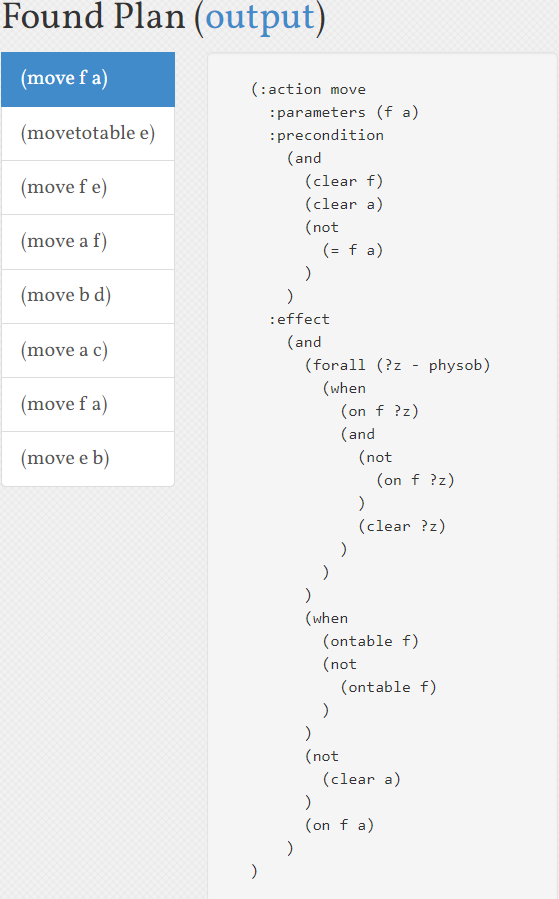
\includegraphics[width=14cm]{result2.png}

%\clearpage
%\bibliography{E:/Papers/LiuLab}
%\bibliographystyle{apalike}
\end{document} 
%%% Local Variables:
%%% mode: latex
%%% TeX-master: t
%%% End:
